\subsection{Non-SD Background}\label{section:star_nonSD}
The background contributions coming from non-diffractive, double-diffractive and central-diffractive events are accounted for by MC simulations. Protons from elastic interactions and beam halo are not included in the simulation process. Background single-diffractive  signatures which are modeled in the Monte Carlo simulations are only coming from :
\begin{itemize}
	\item forward protons produced in the SD, CD or DD diffractive systems or through non-diffractive  QCD,
	\item reconstructed tracks coming from showering.
\end{itemize}
Figure~\ref{fig:nonSDxit} shows the uncorrected $\xi$ and $t$ data compared to various MC models: PYTHIA 8 A2 (MBR), PYTHIA 8 A2 (MBR-tuned) and EPOS, where the MC distributions are split into SD, ND, DD and CD components. For EPOS low mass excitation of the proton remnant (SD') is separated from the ND events. Additionally, the accidental background is also shown. Without arbitrary suppression of diffractive cross sections at large $\xi$ PYTHIA8 A2 (MBR-tuned) predictions agree much better with the data and result also in a suppression of non-SD events. EPOS describes data better than PYTHIA8 but shows a dominant contribution of SD' events. All MCs predict significant non-SD background at large $\xi$, thereby  the analysis was limited to $\xi < 0.2$. 

\begin{figure}[h!]
	\centering
	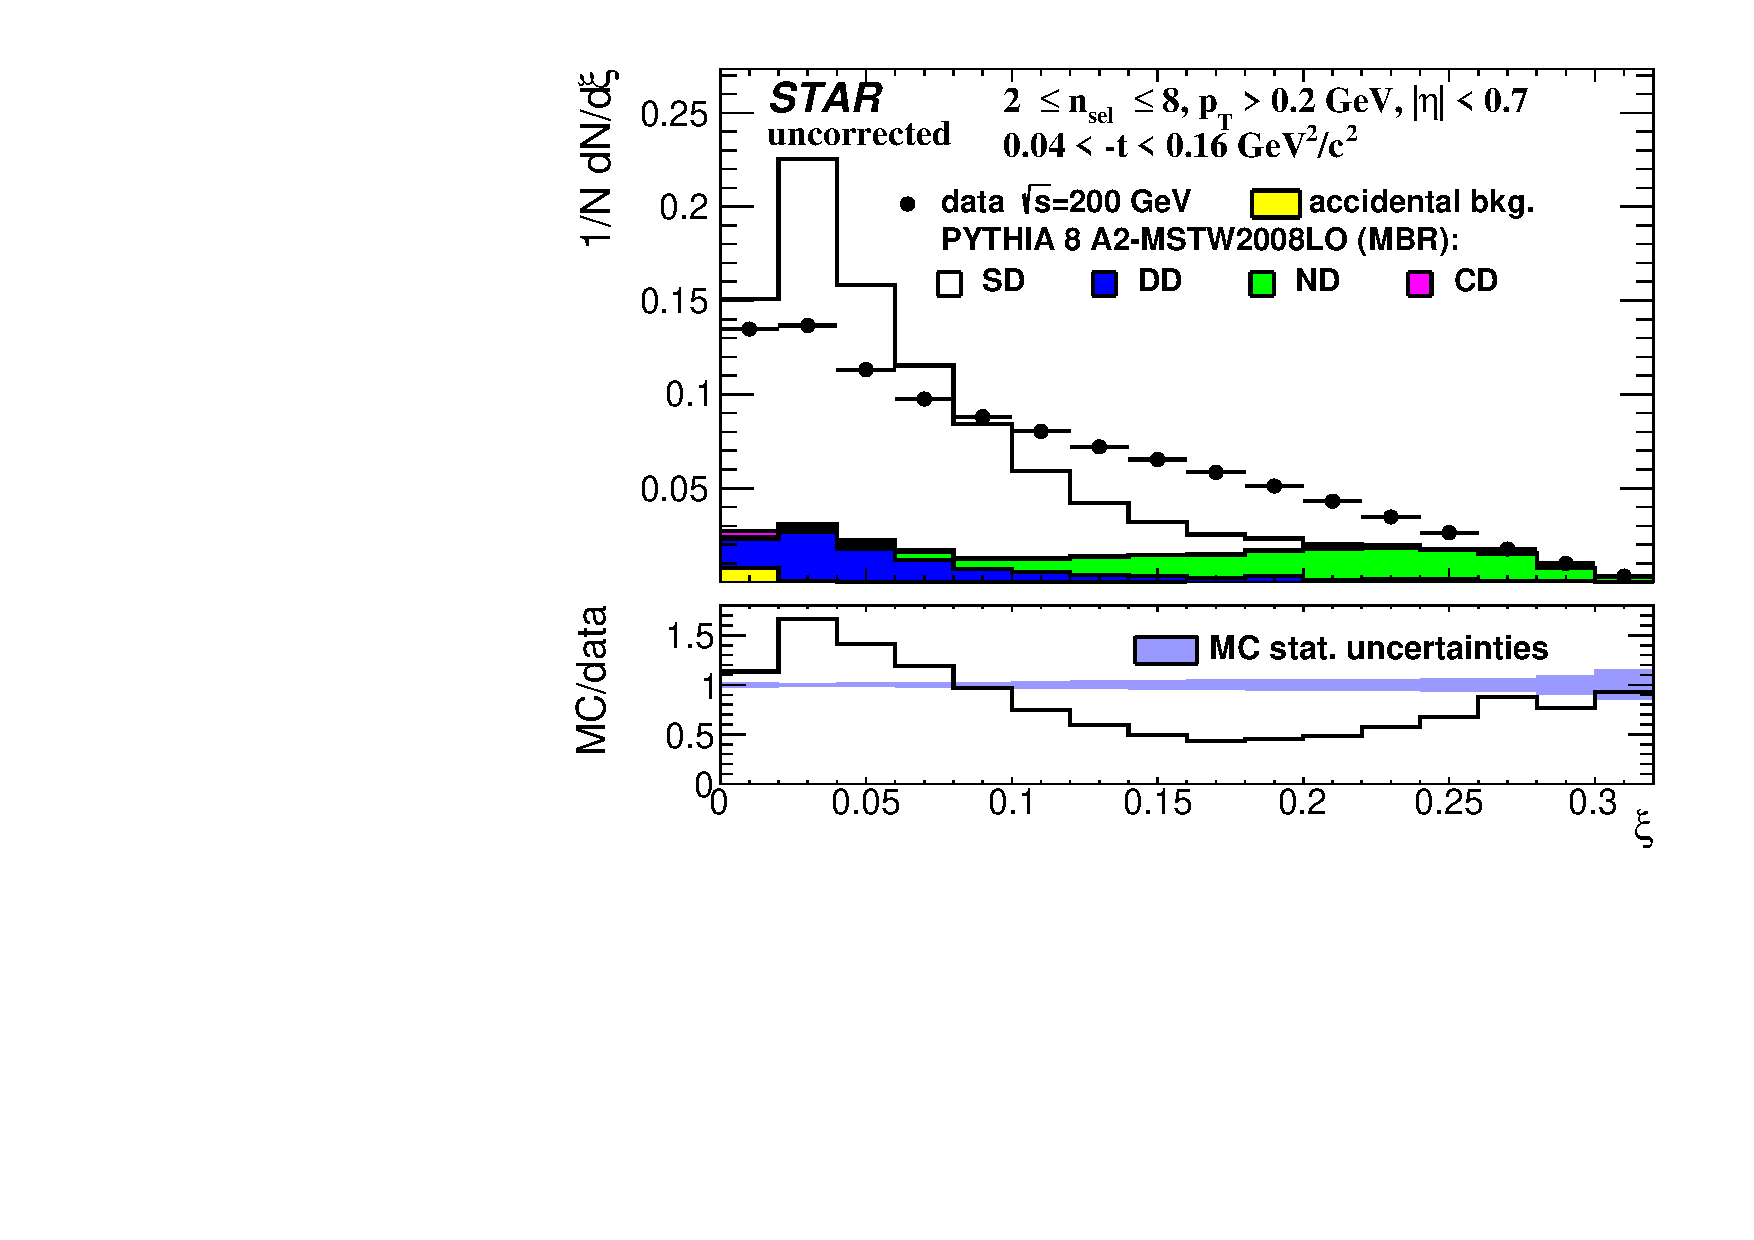
\includegraphics[width=.49\textwidth,page=1]{chapters/chrgSTAR/img/nonSD/SDT_pythia_xi0_RP_starsim_xi.pdf}
	\hfill
	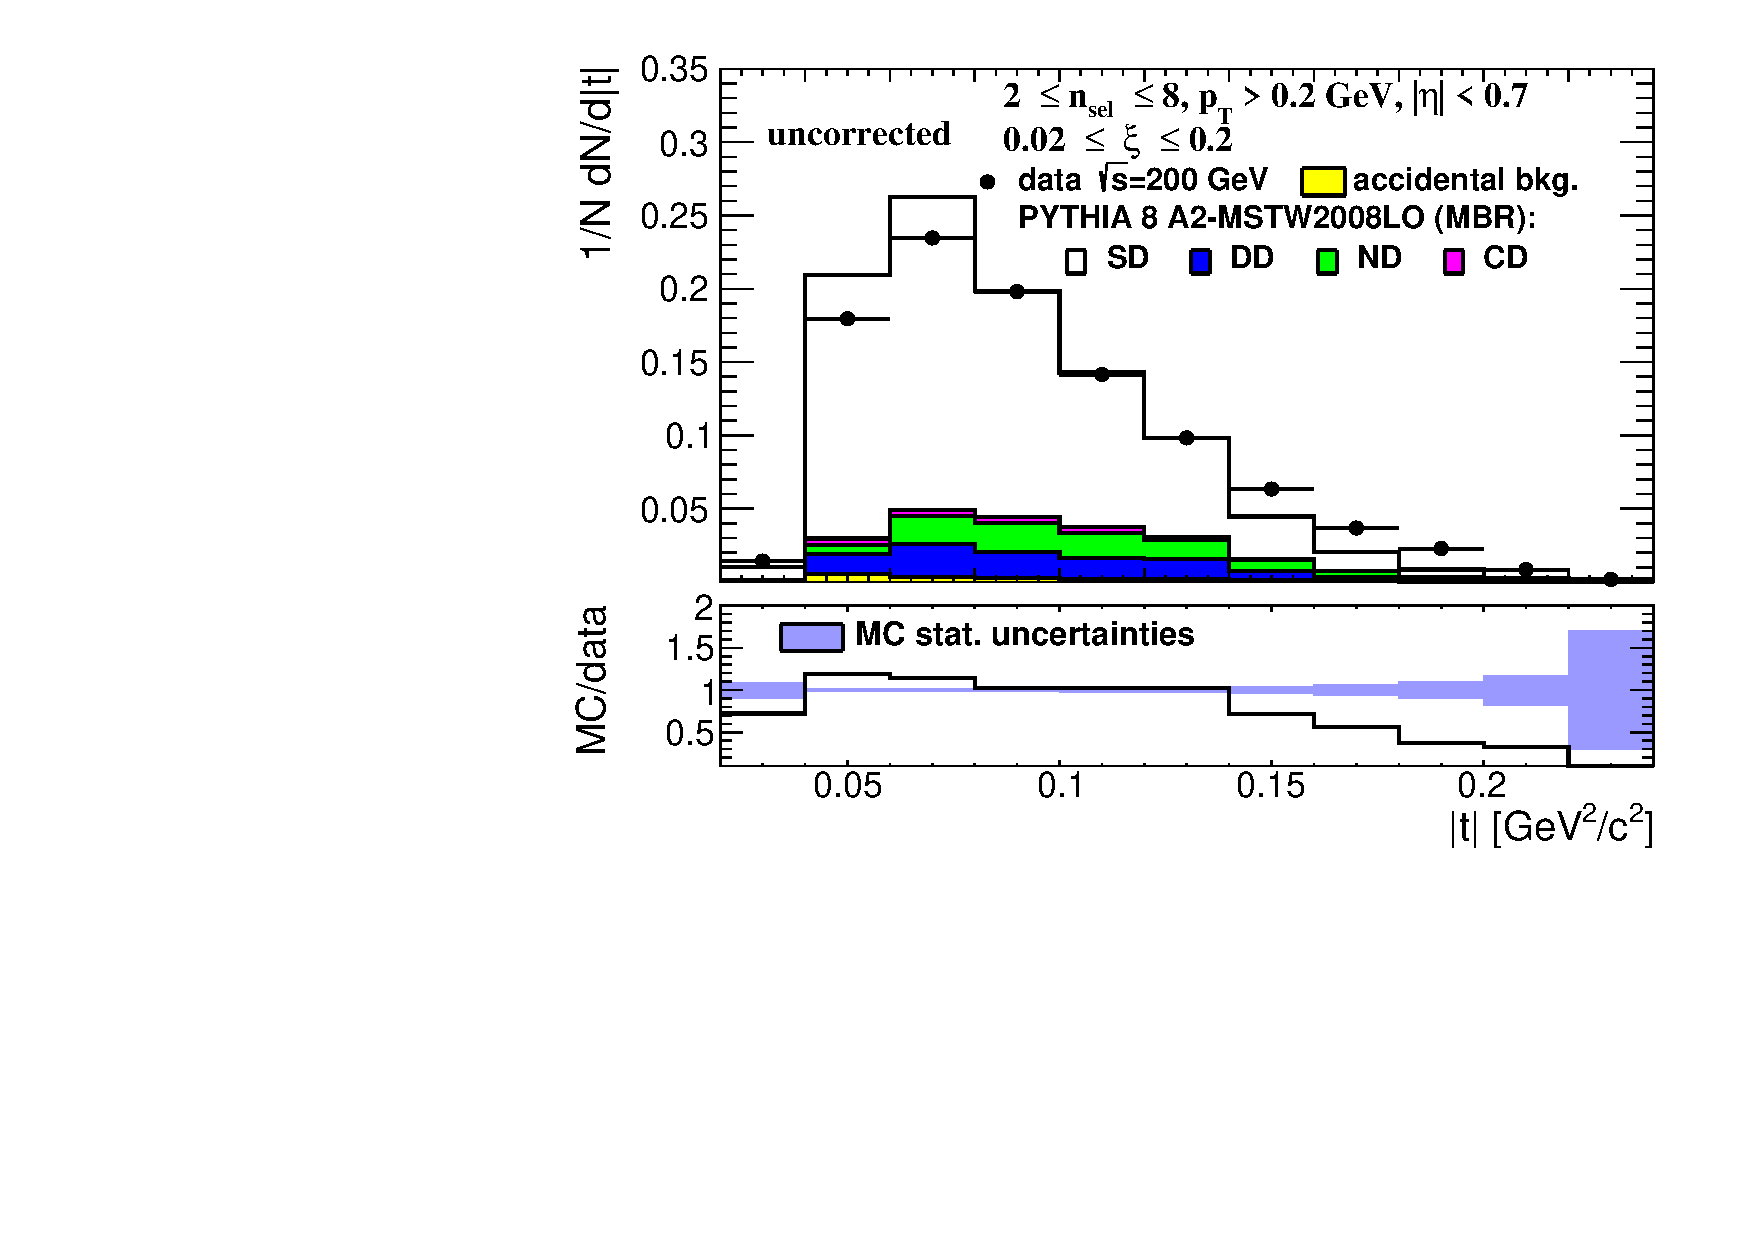
\includegraphics[width=.49\textwidth,page=1]{chapters/chrgSTAR/img/nonSD/SDT_pythia_xi0_RP_starsim_t.pdf}
	\newline
	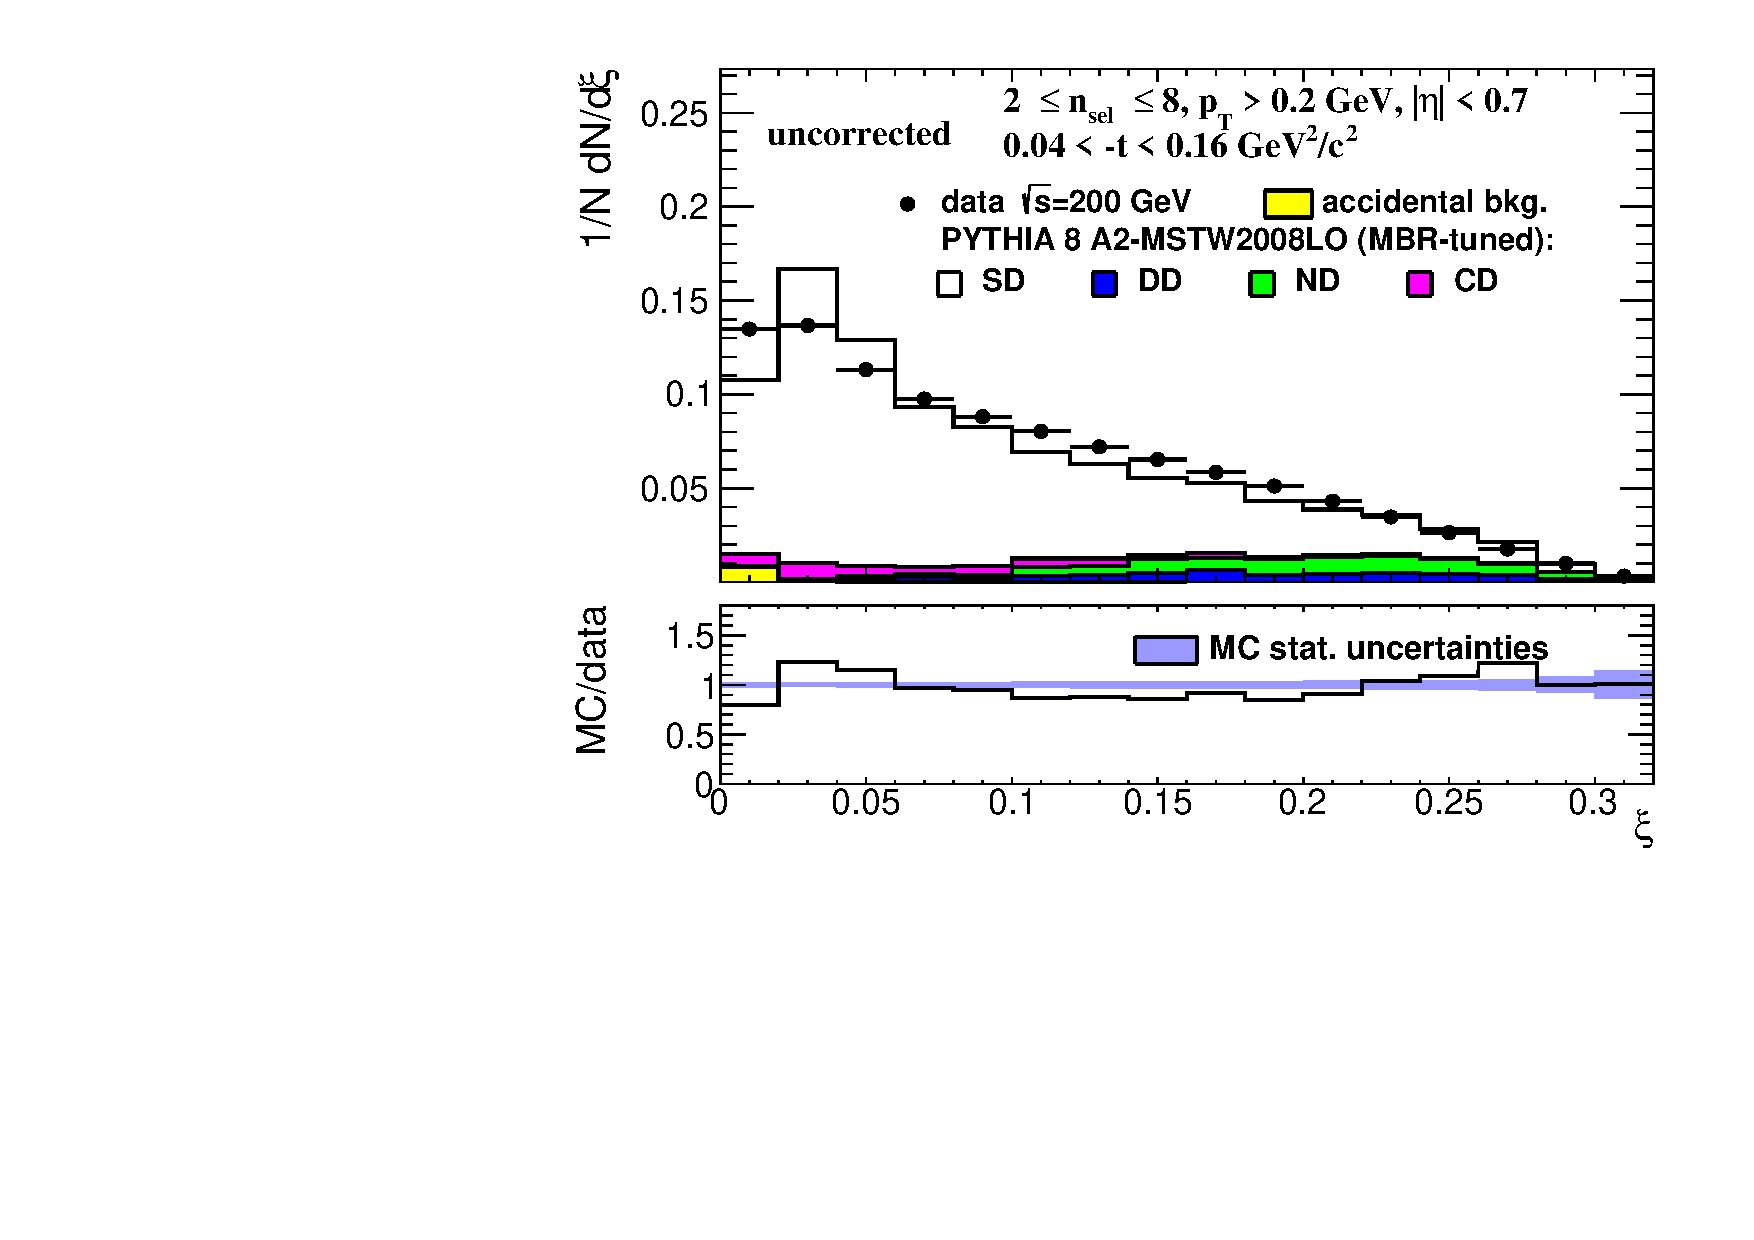
\includegraphics[width=.49\textwidth,page=1]{chapters/chrgSTAR/img/nonSD/SDT_pythia_xi0_option2_RP_starsim_xi.pdf}
	\hfill
	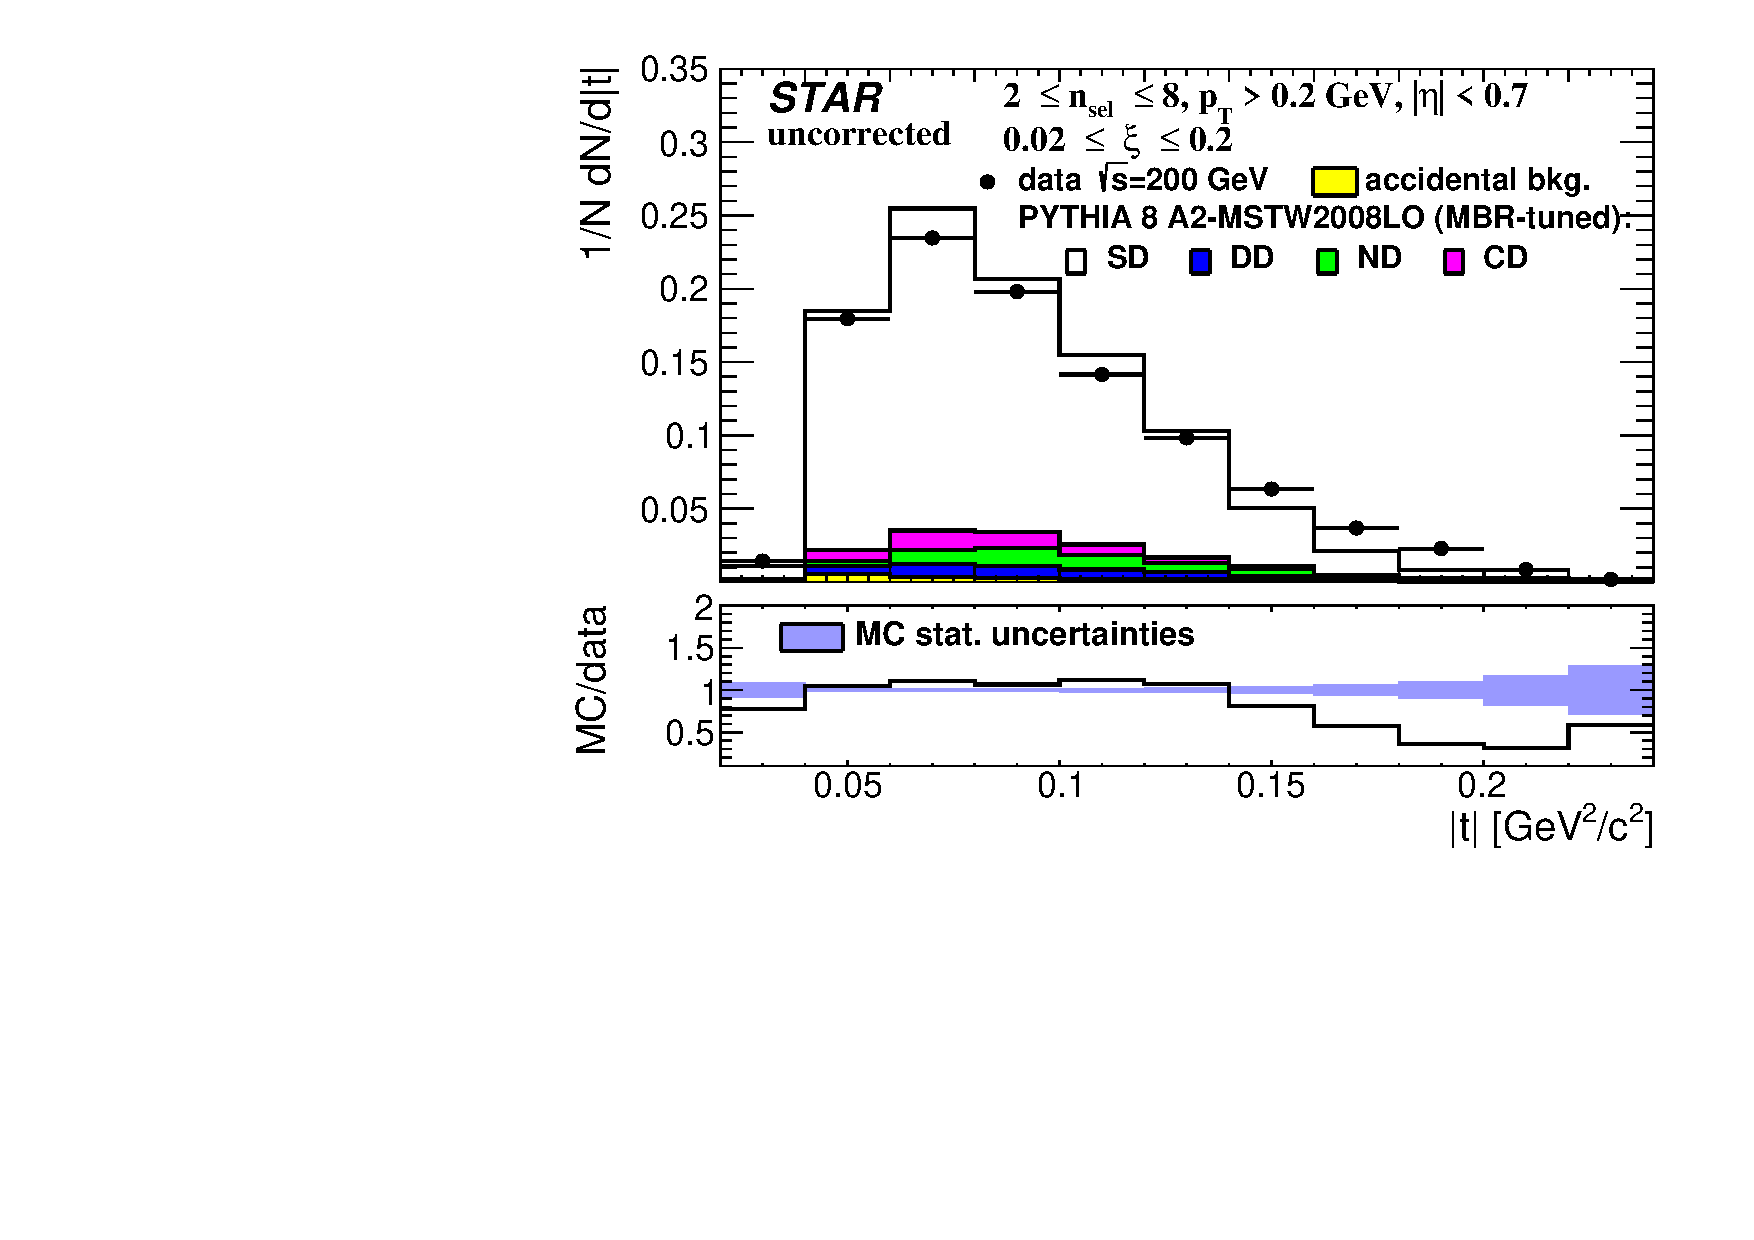
\includegraphics[width=.49\textwidth,page=1]{chapters/chrgSTAR/img/nonSD/SDT_pythia_xi0_option2_RP_starsim_t.pdf}
	\newline
	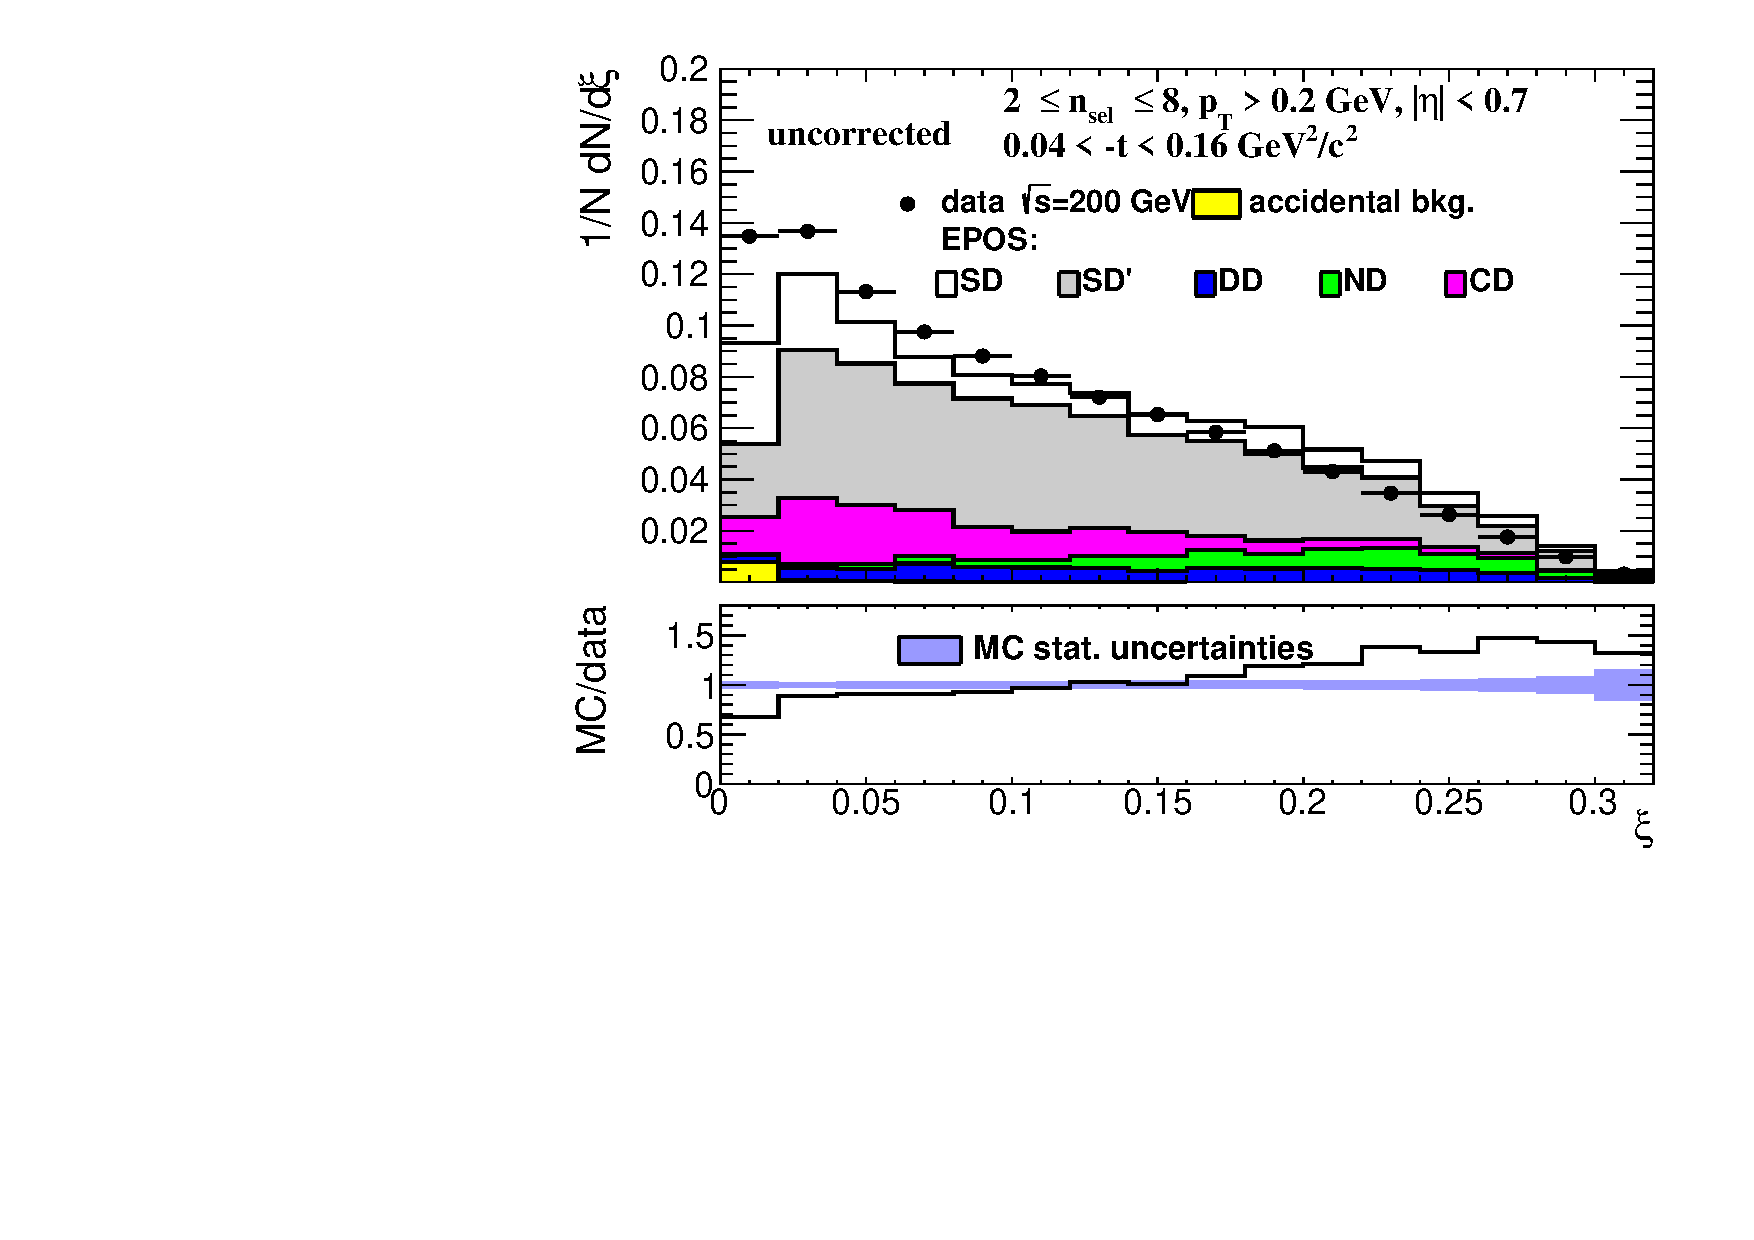
\includegraphics[width=.49\textwidth,page=1]{chapters/chrgSTAR/img/nonSD/SDT_epos_xi0_RP_starsim_xi.pdf}
	\hfill
	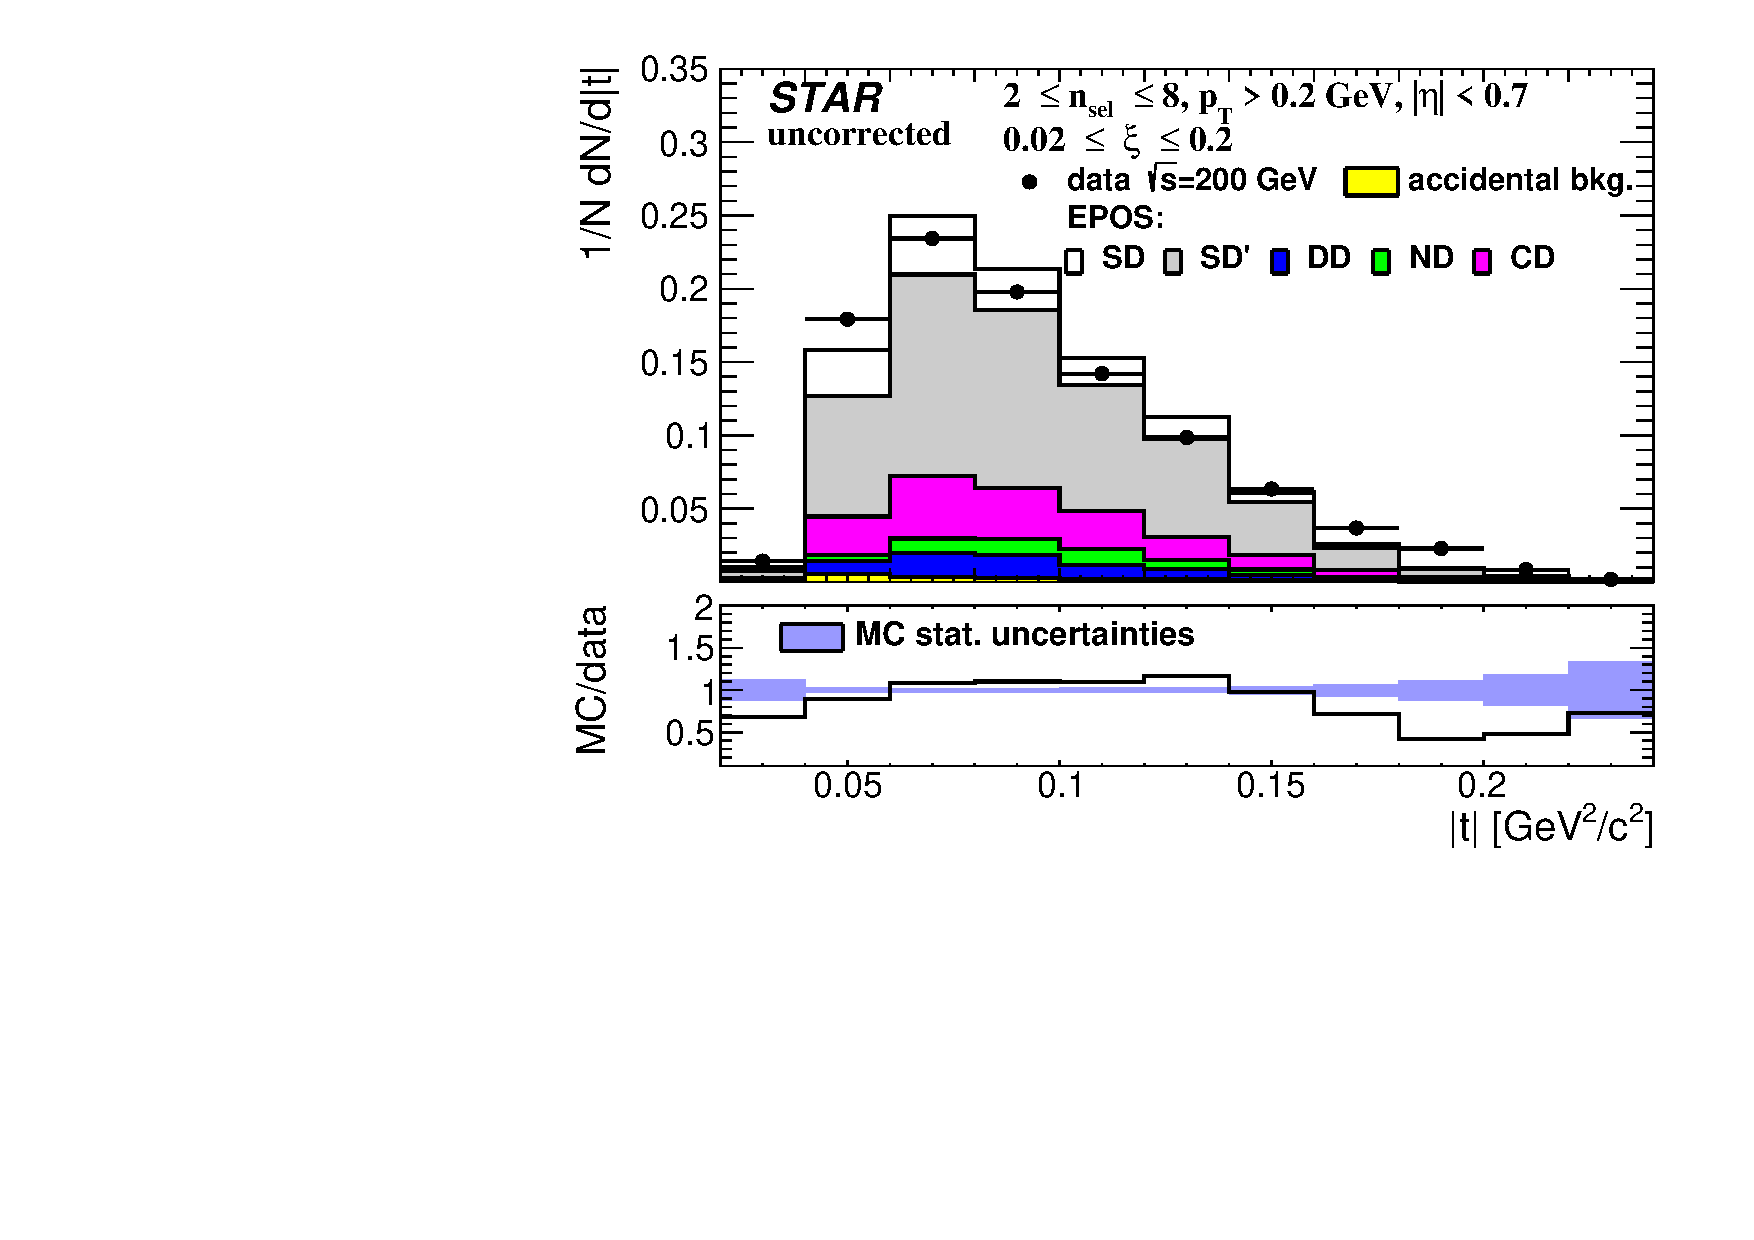
\includegraphics[width=.49\textwidth,page=1]{chapters/chrgSTAR/img/nonSD/SDT_epos_xi0_RP_starsim_t.pdf}
	%
	\caption[Uncorrected distributions of data compared to various MC models: PYTHIA8 A2 (MBR), PYTHIA8 A2 (MBR-tuned) and  EPOS, as a function of $\xi$ and $|t|$.]{Uncorrected distributions of data compared to various MC models: (top) PYTHIA8 A2 (MBR), (middle) PYTHIA8 A2 (MBR-tuned) and (bottom) EPOS, as a function of $\xi$ (left column) and $|t|$ (right column). Both data and MC are scaled by the respective numbers of events in the samples.}
	\label{fig:nonSDxit}
\end{figure}
\FloatBarrier
On the other hand, \cref{fig:nonSDnsel,fig:nonSDpt,fig:nonSDera} show the uncorrected distributions of variables used in the later analysis: $n_{sel}$, $p_T$ an $\bar{\eta}$. The background contributions from non-SD interactions differ a bit between each other, i.e. EPOS predicts significantly larger CD contribution, whereas DD and ND are suppressed in PYTHIA 8 A2 (MBR-tuned).  As a result PYTHIA~8~A2~(MBR) was used as the default model  of non-SD with systematic uncertainty $\pm50\%$, which covers all differences between models. Moreover, SD' in EPOS was not subtracted but used separately for comparisons.
\captionsetup{format=plain,indention=0pt,justification=justified}
\begin{figure}[h!]
	\centering
	\begin{subfigure}{.49\textwidth}
		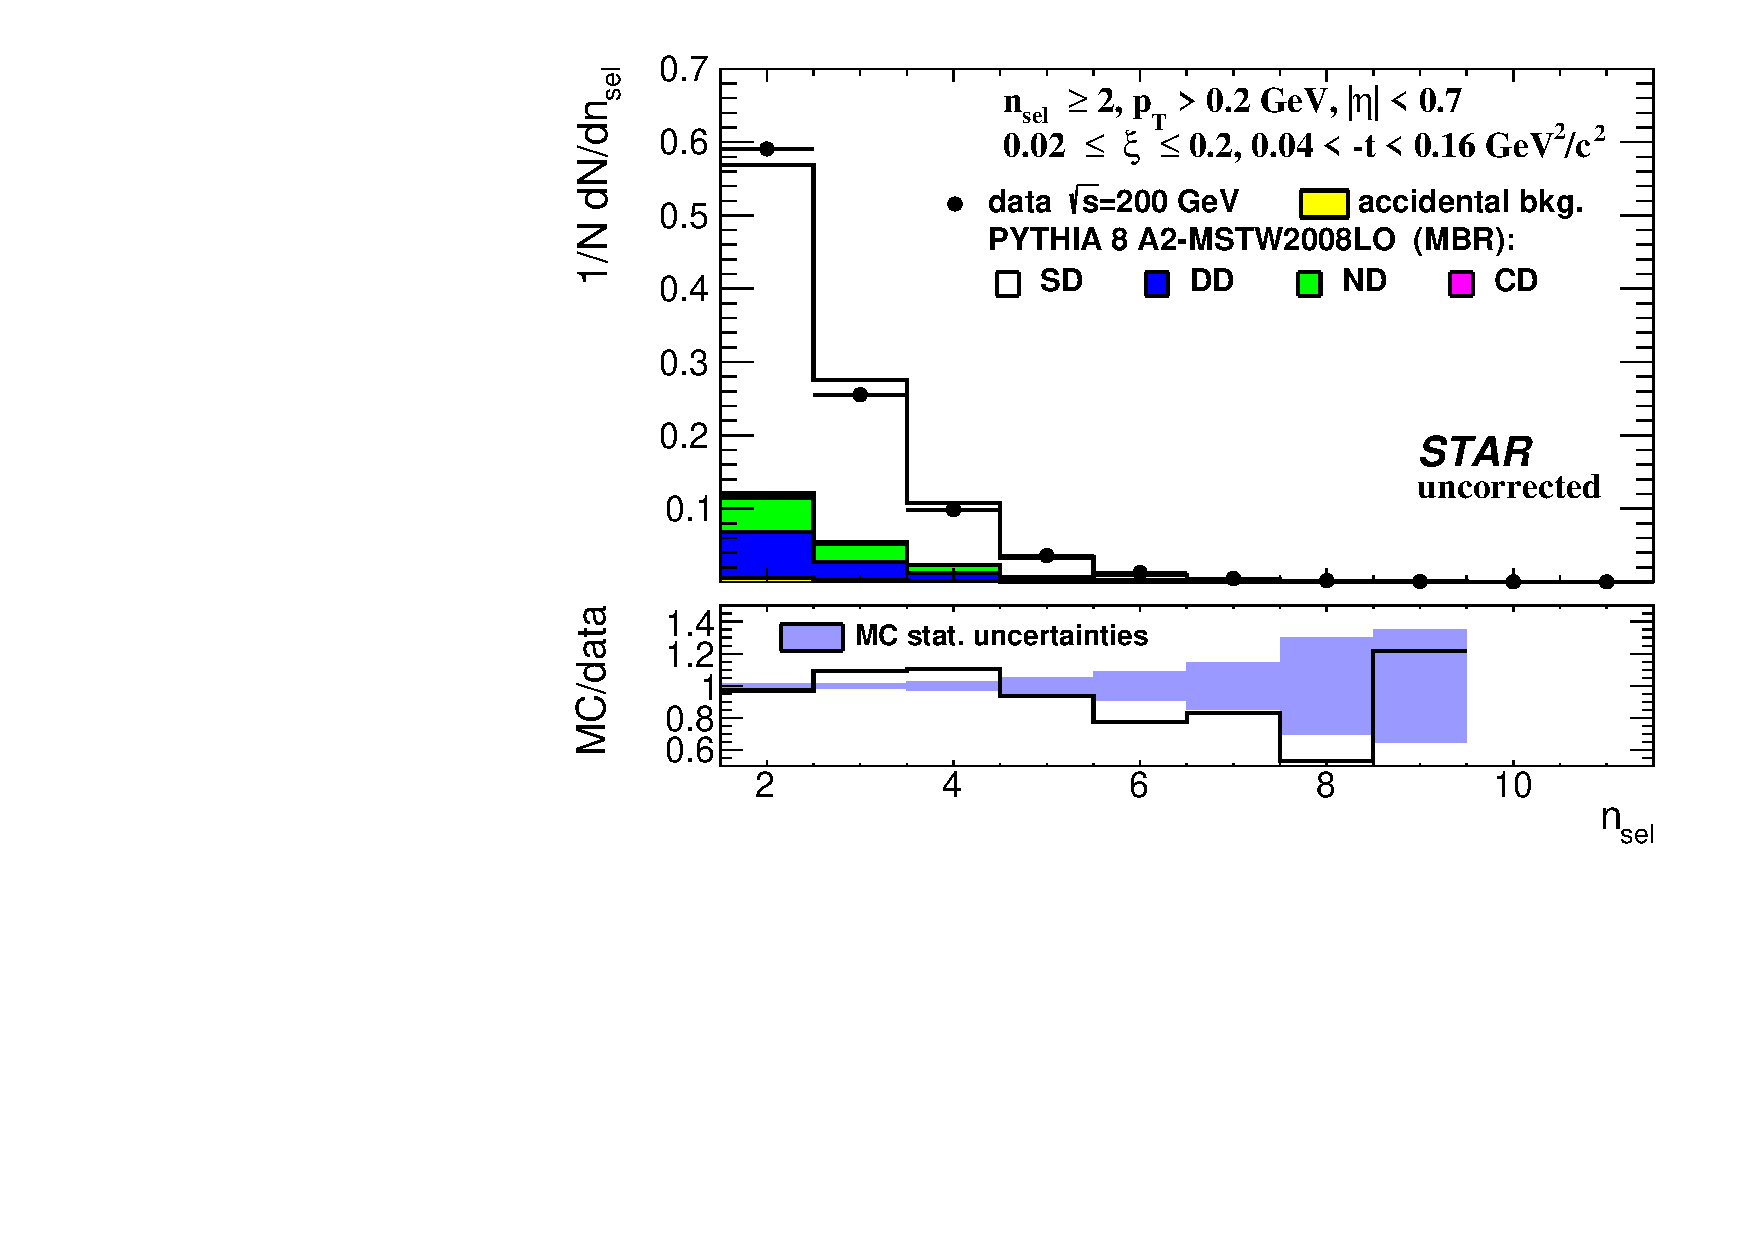
\includegraphics[width=\linewidth, page=1]{chapters/chrgSTAR/img/nonSD/chrg/SDT_pythia_xi0_RP_starsim_nsel.pdf}
	\end{subfigure}
	\begin{subfigure}{.49\textwidth}
		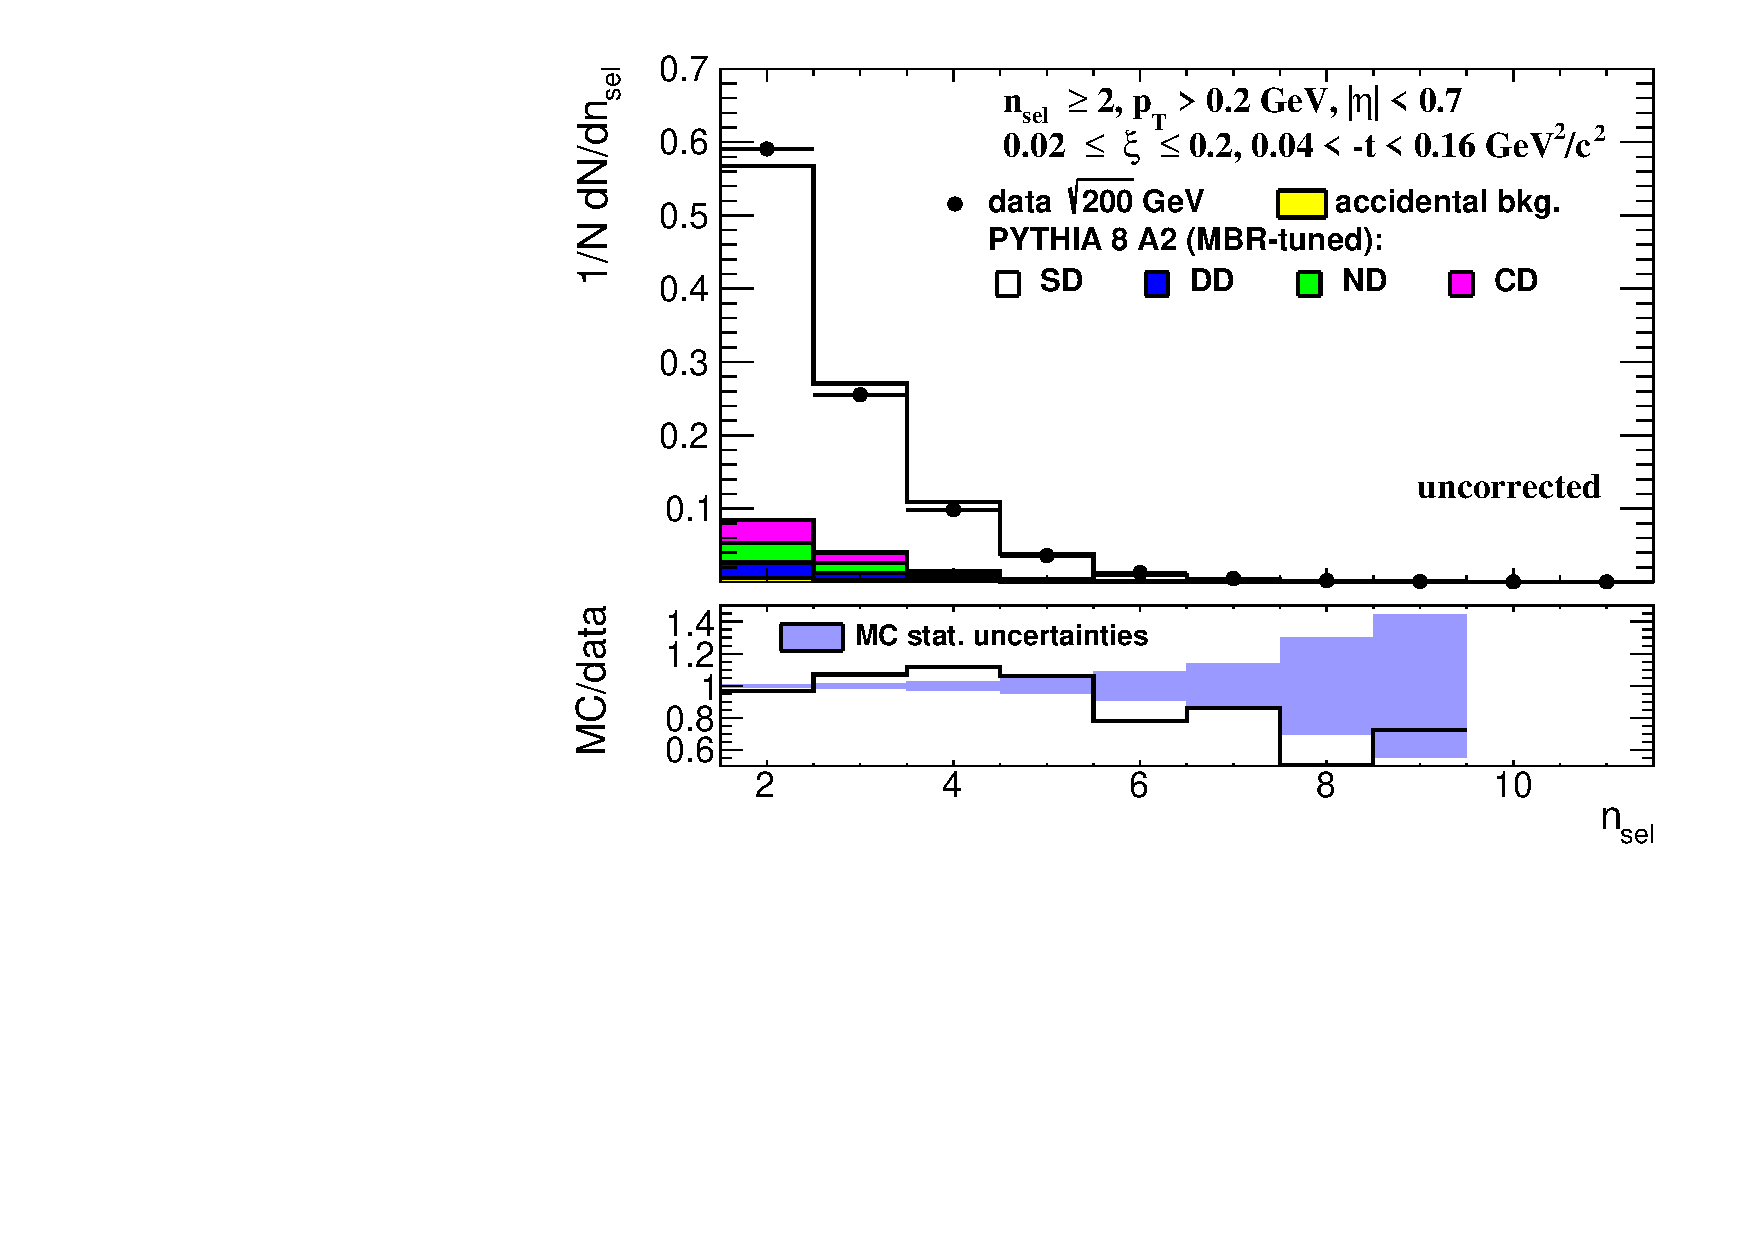
\includegraphics[width=\linewidth, page=1]{chapters/chrgSTAR/img/nonSD/chrg/SDT_pythia_xi0_option2_RP_starsim_nsel.pdf}
	\end{subfigure}
	\begin{subfigure}{.49\textwidth}
		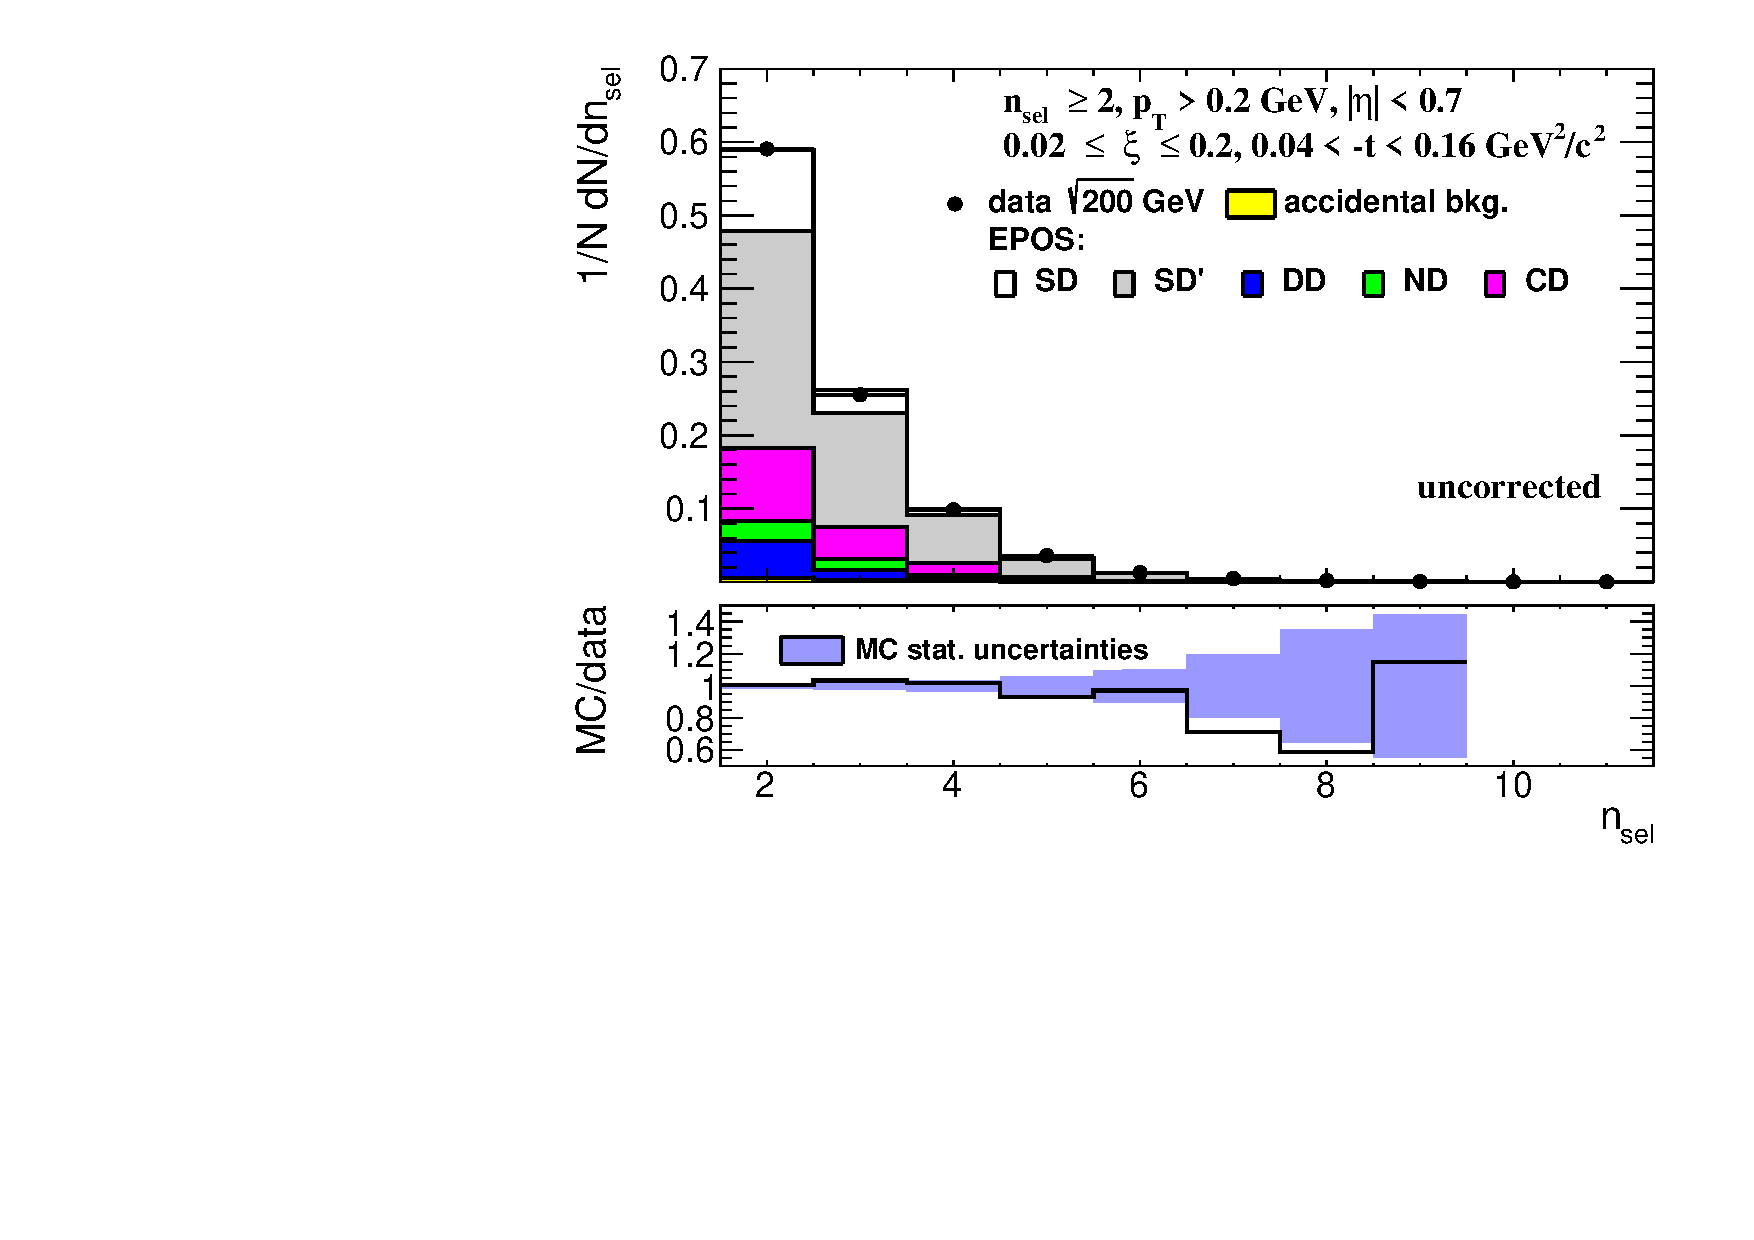
\includegraphics[width=\linewidth, page=1]{chapters/chrgSTAR/img/nonSD/chrg/SDT_epos_xi0_RP_starsim_nsel.pdf}
	\end{subfigure}
	\begin{minipage}{.49\textwidth}
		\caption[Uncorrected distributions of data compared to various MC models: PYTHIA8 A2 (MBR), PYTHIA8 A2 (MBR-tuned) and EPOS, as a function of $n_{sel}$.]{Uncorrected distributions of data compared to various MC models: (top left) PYTHIA8 A2 (MBR), (top right) PYTHIA8 A2 (MBR-tuned) and (bottom) EPOS, as a function of $n_{sel}$. Both data and MC are scaled by the respective numbers of events in the samples.}
		\label{fig:nonSDnsel}
	\end{minipage}
	
\end{figure}
\begin{figure}[h!]
%	\vspace{-0.5cm}
	\centering
	\begin{subfigure}{.45\textwidth}
		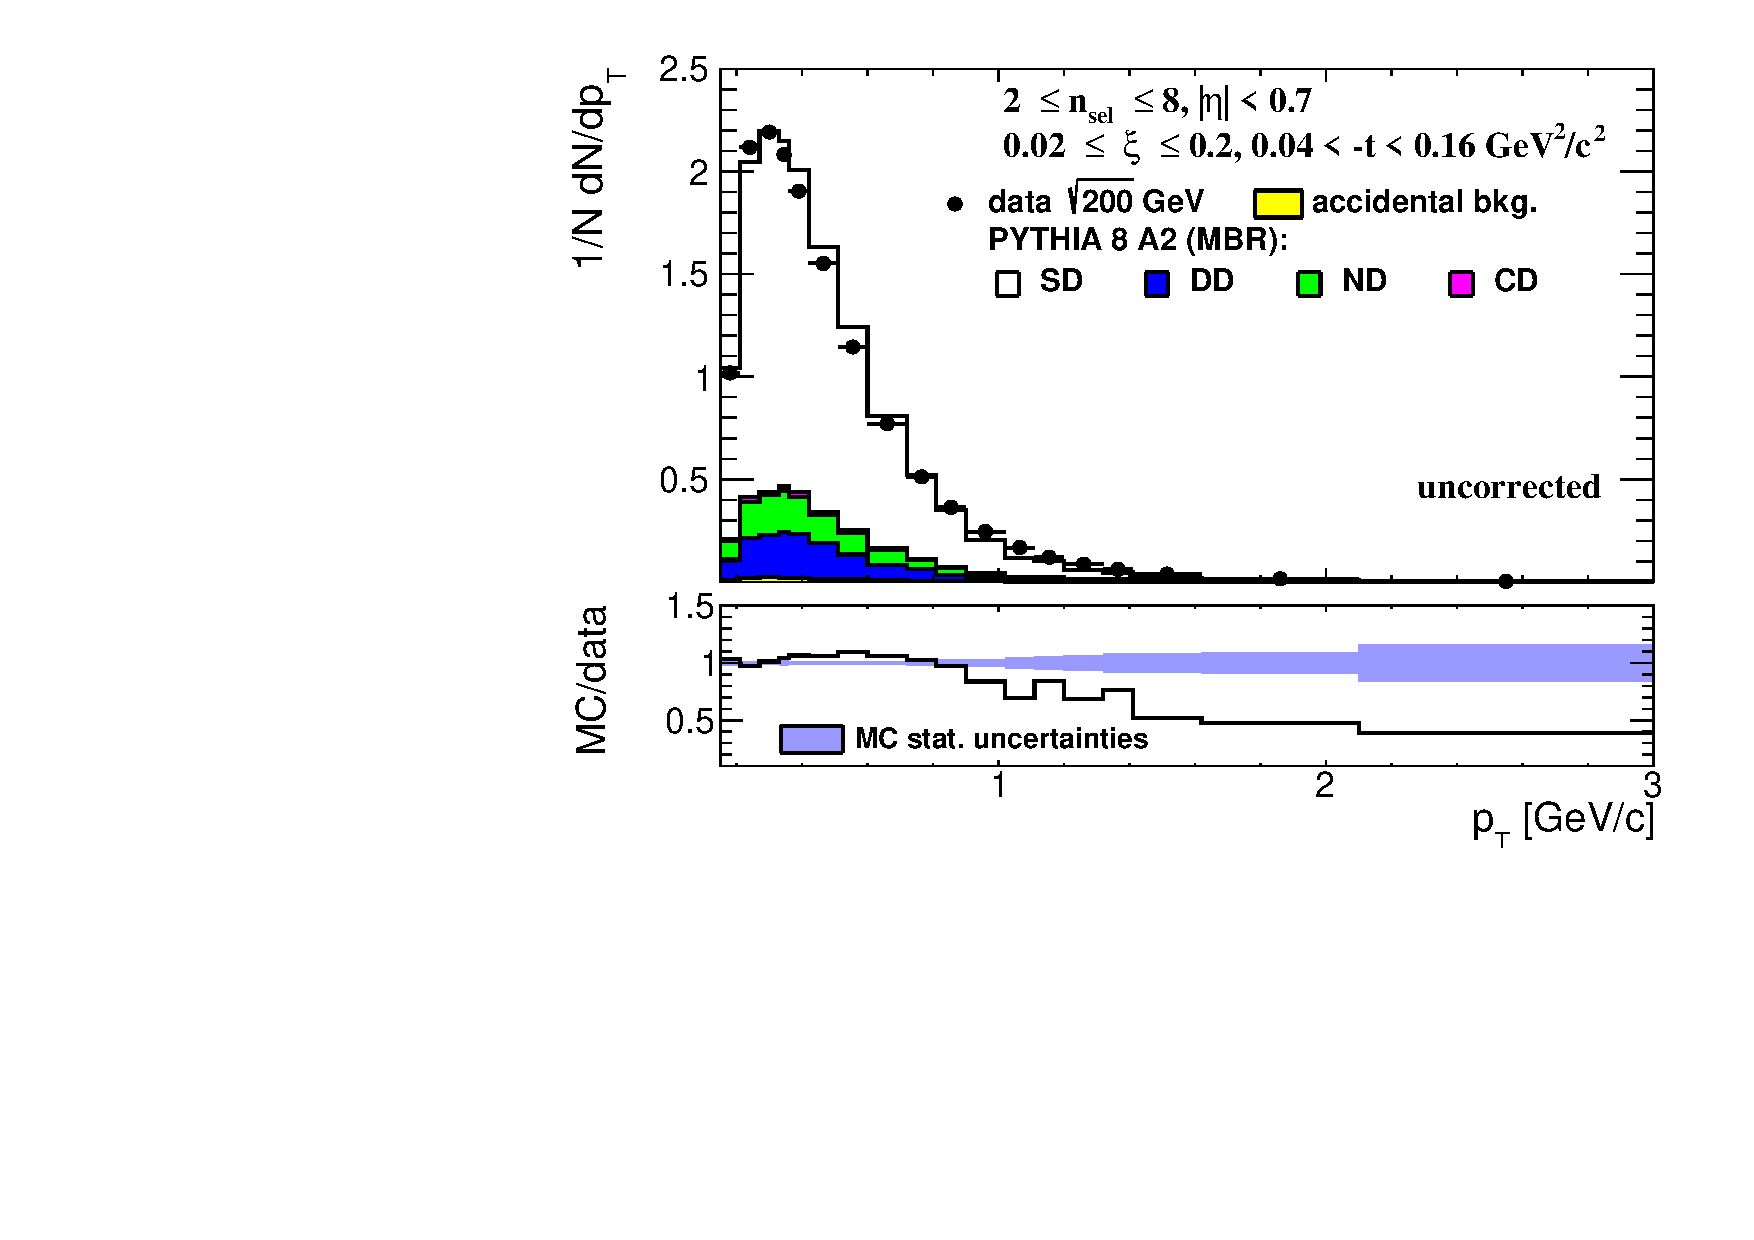
\includegraphics[width=\linewidth, page=1]{chapters/chrgSTAR/img/nonSD/chrg/SDT_pythia_xi0_RP_starsim_pt.pdf}
	\end{subfigure}
	\begin{subfigure}{.45\textwidth}
		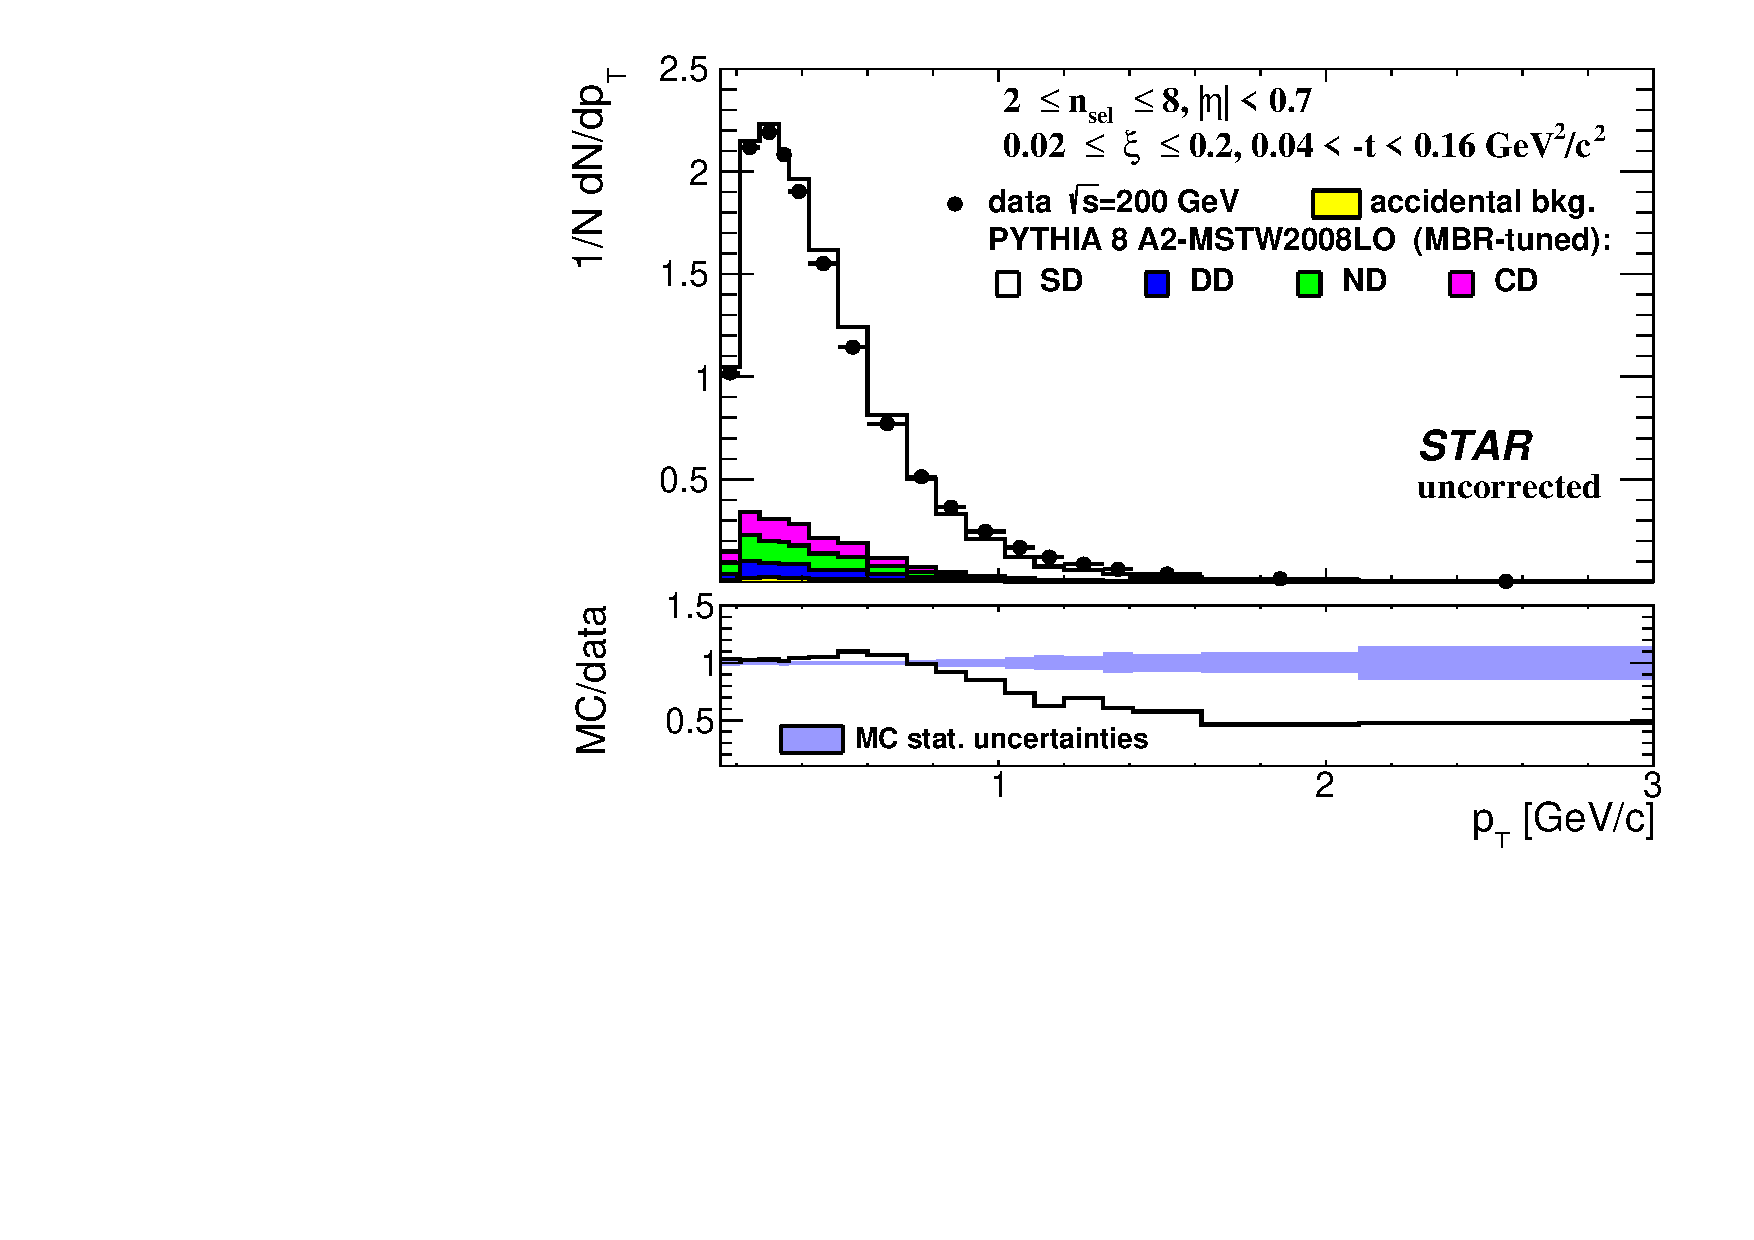
\includegraphics[width=\linewidth, page=1]{chapters/chrgSTAR/img/nonSD/chrg/SDT_pythia_xi0_option2_RP_starsim_pt.pdf}
	\end{subfigure}
	\begin{subfigure}{.45\textwidth}
		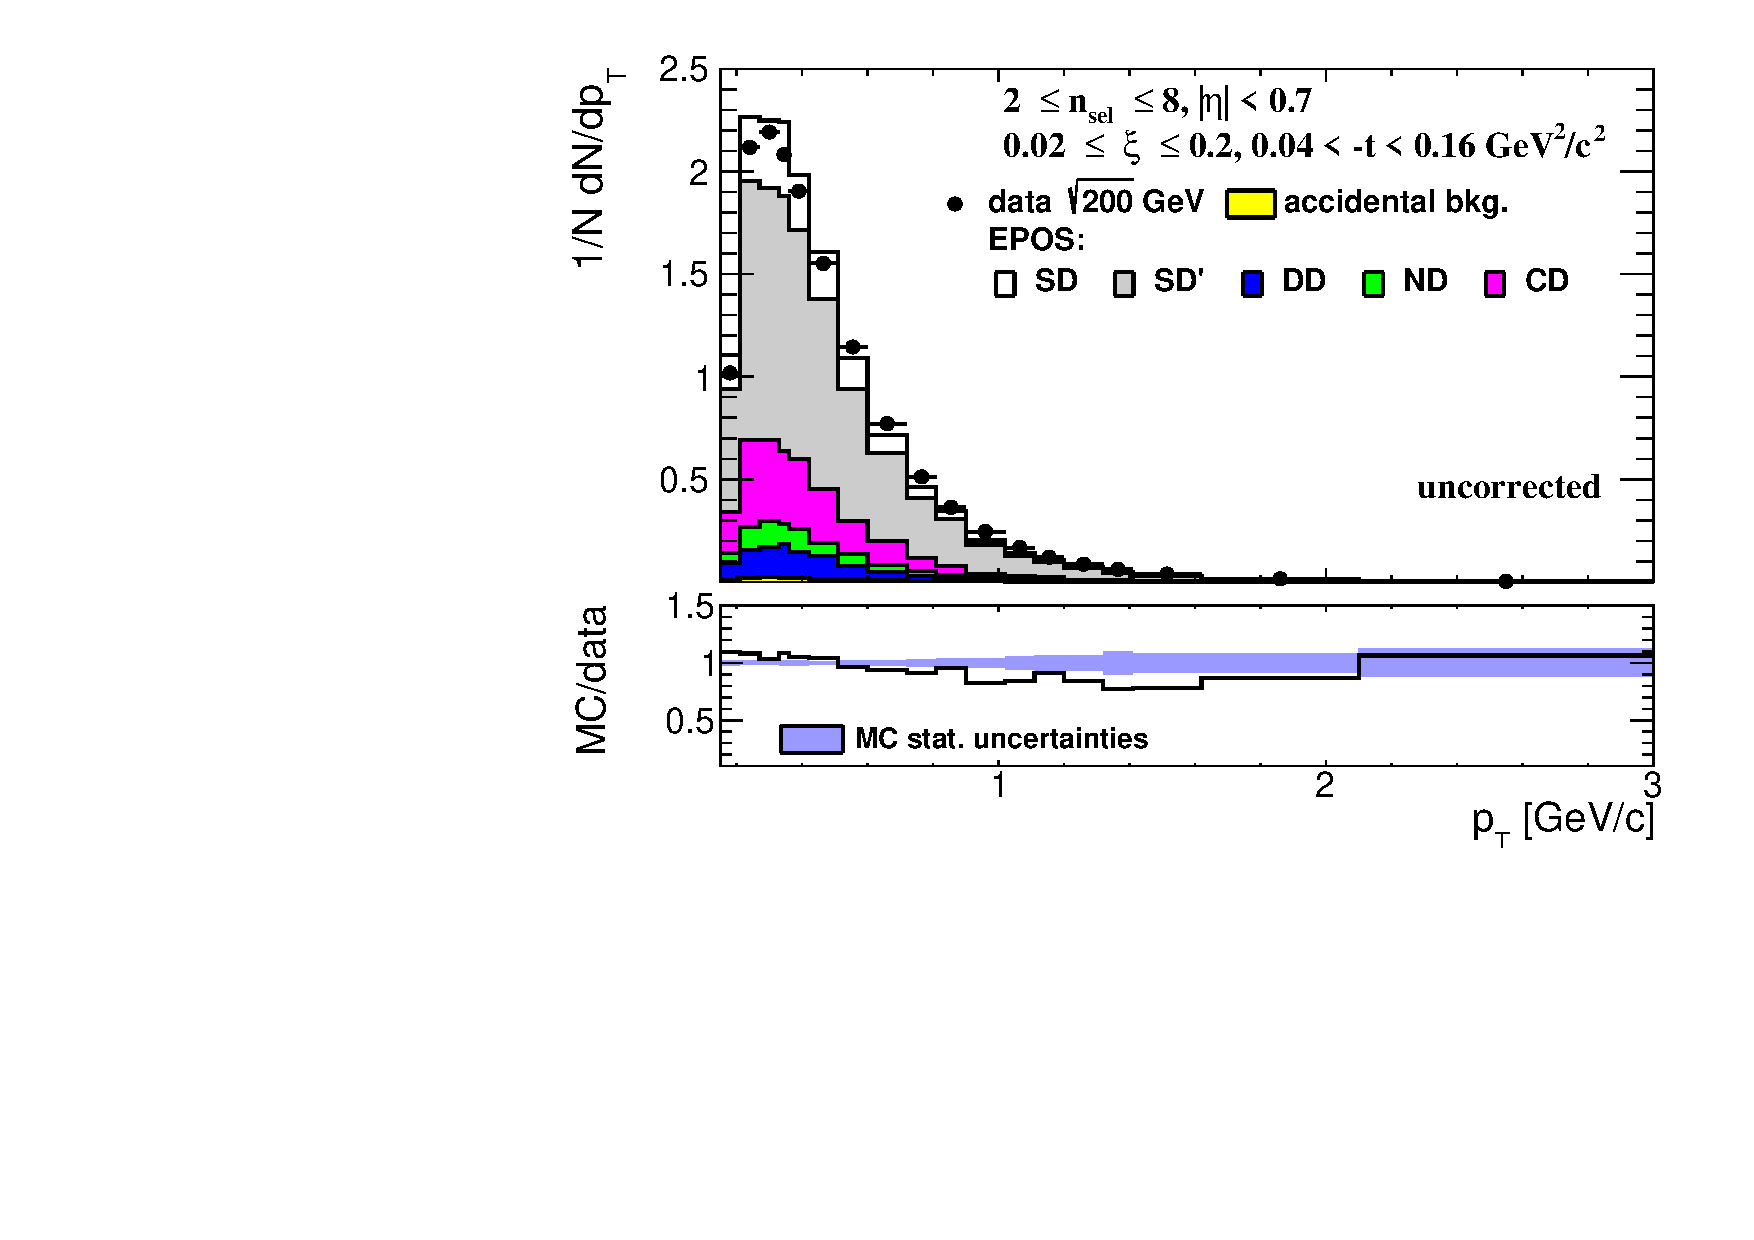
\includegraphics[width=\linewidth, page=1]{chapters/chrgSTAR/img/nonSD/chrg/SDT_epos_xi0_RP_starsim_pt.pdf}
	\end{subfigure}
	\begin{minipage}{.45\textwidth}
		\caption[Uncorrected distributions of data compared to various MC models: PYTHIA8 A2 (MBR), PYTHIA8 A2 (MBR-tuned) and EPOS, as a function of $p_T$.]{Uncorrected distributions of data compared to various MC models: (top left) PYTHIA8 A2 (MBR), (top right) PYTHIA8 A2 (MBR-tuned) and (bottom) EPOS, as a function of $p_T$. Both data and MC are scaled by the respective numbers of events in the samples.}
		\label{fig:nonSDpt}
	\end{minipage}
	
\end{figure}

\begin{figure}[h!]
%	\vspace{-0.5cm}
	\centering
	\begin{subfigure}{.45\textwidth}
		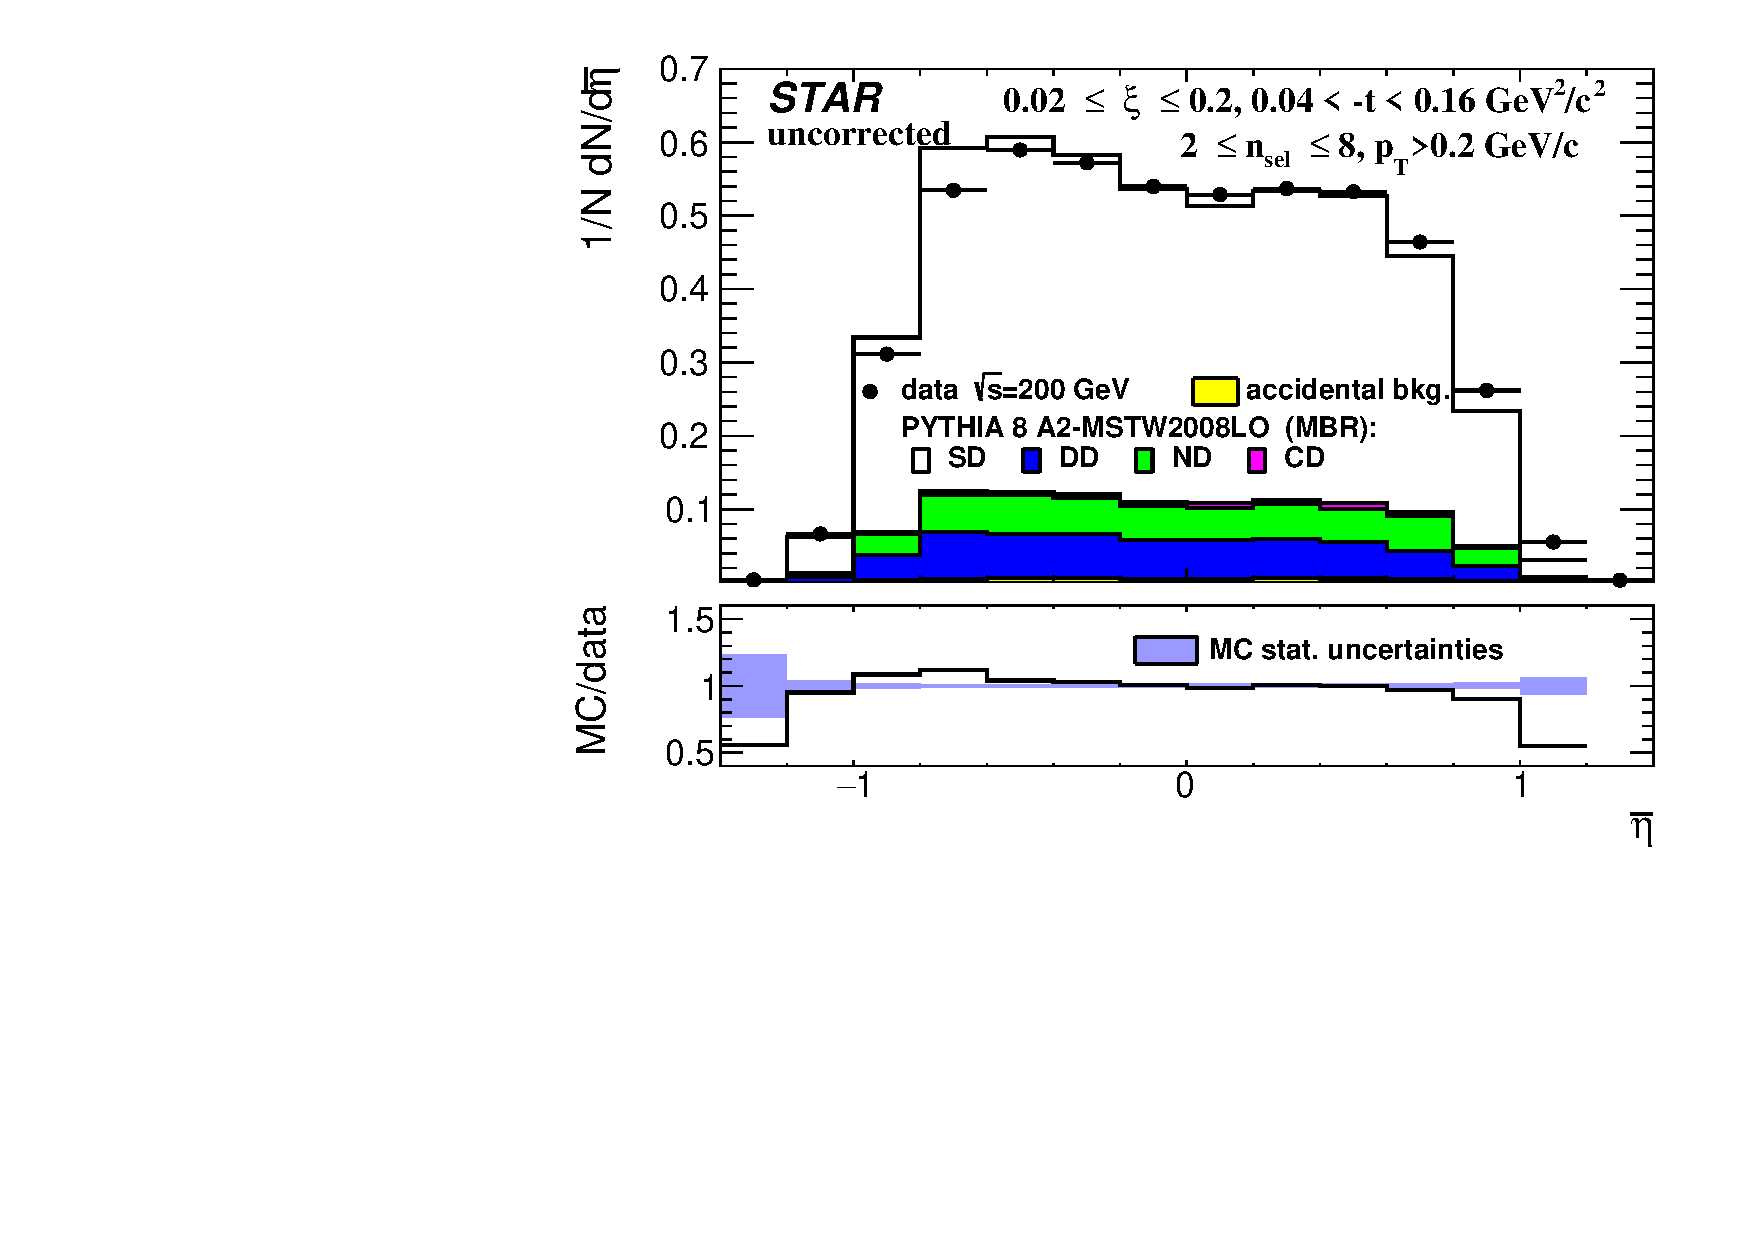
\includegraphics[width=\linewidth, page=1]{chapters/chrgSTAR/img/nonSD/chrg/SDT_pythia_xi0_RP_starsim_eta.pdf}
	\end{subfigure}
	\begin{subfigure}{.45\textwidth}
		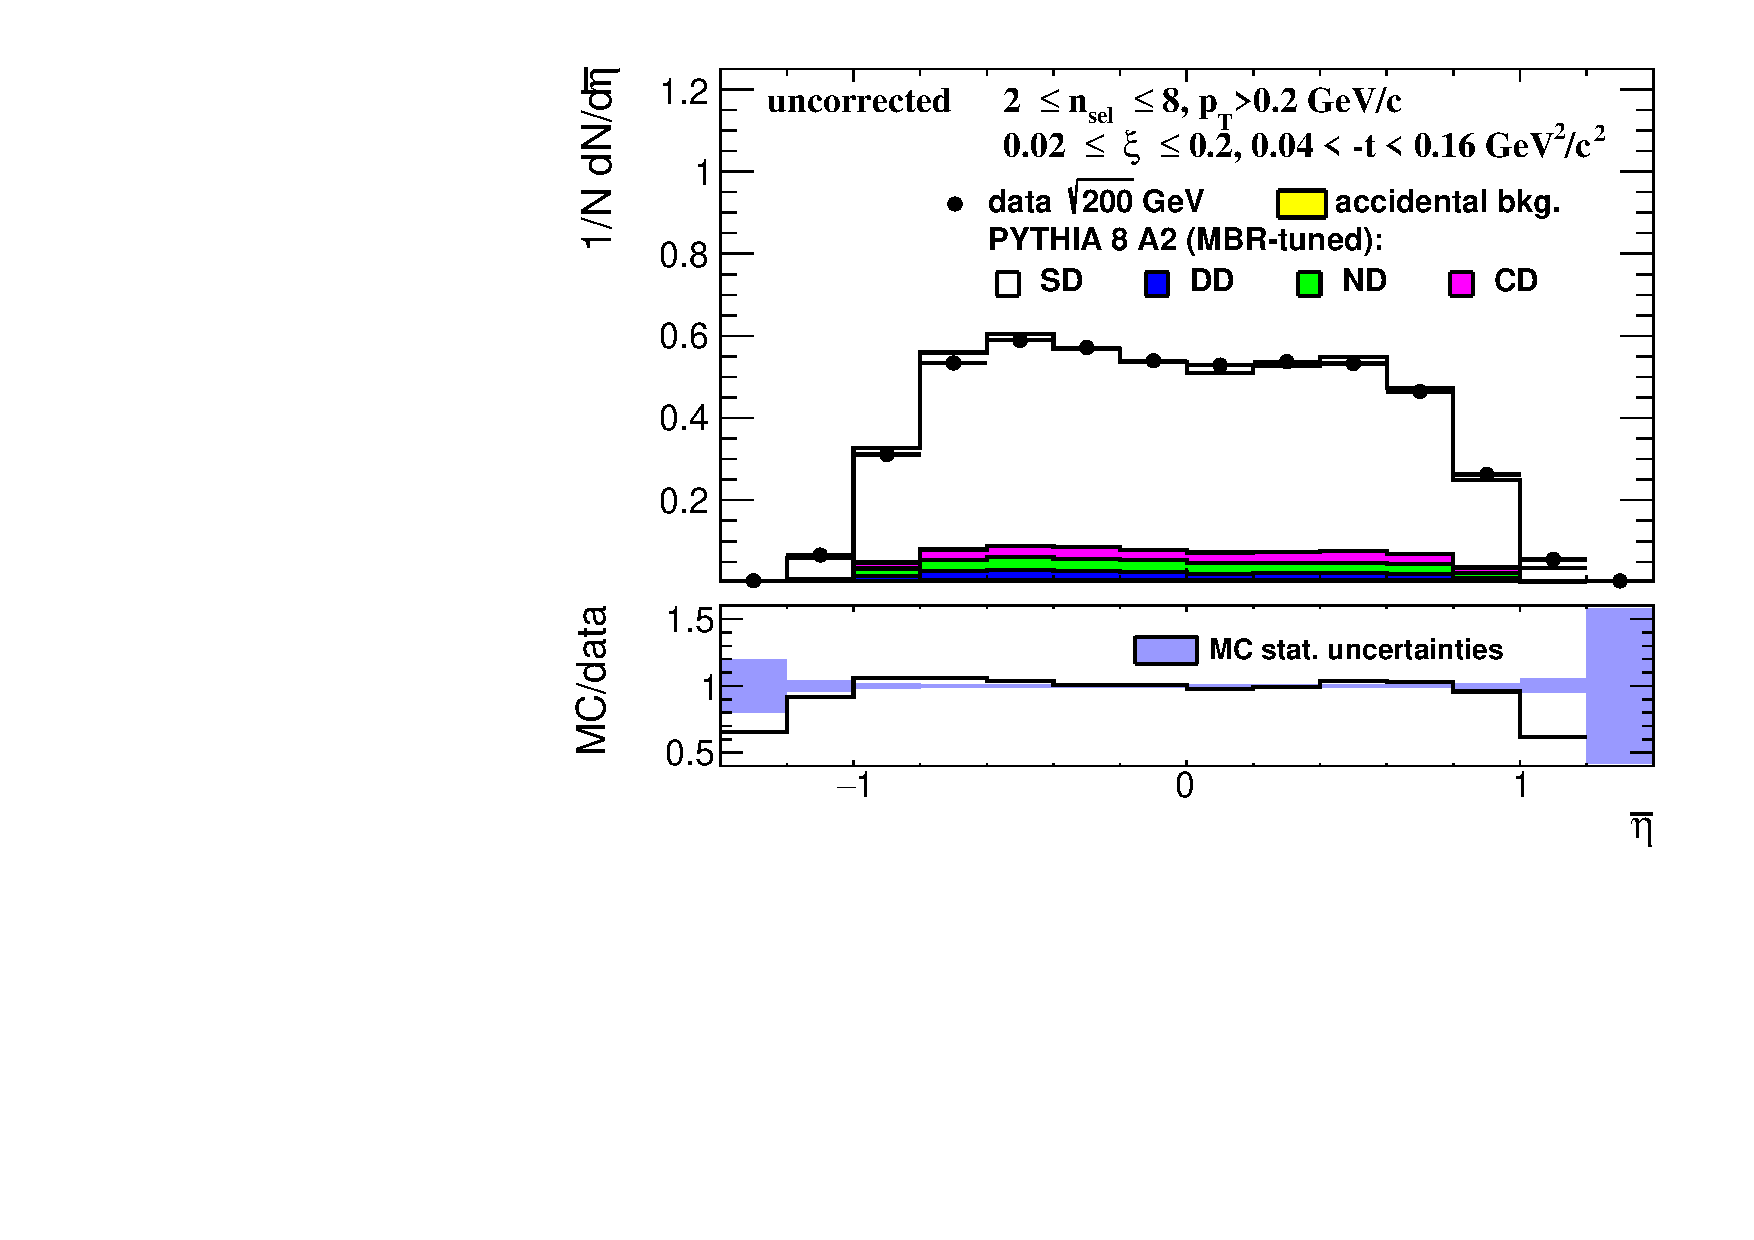
\includegraphics[width=\linewidth, page=1]{chapters/chrgSTAR/img/nonSD/chrg/SDT_pythia_xi0_option2_RP_starsim_eta.pdf}
	\end{subfigure}
	\begin{subfigure}{.45\textwidth}
		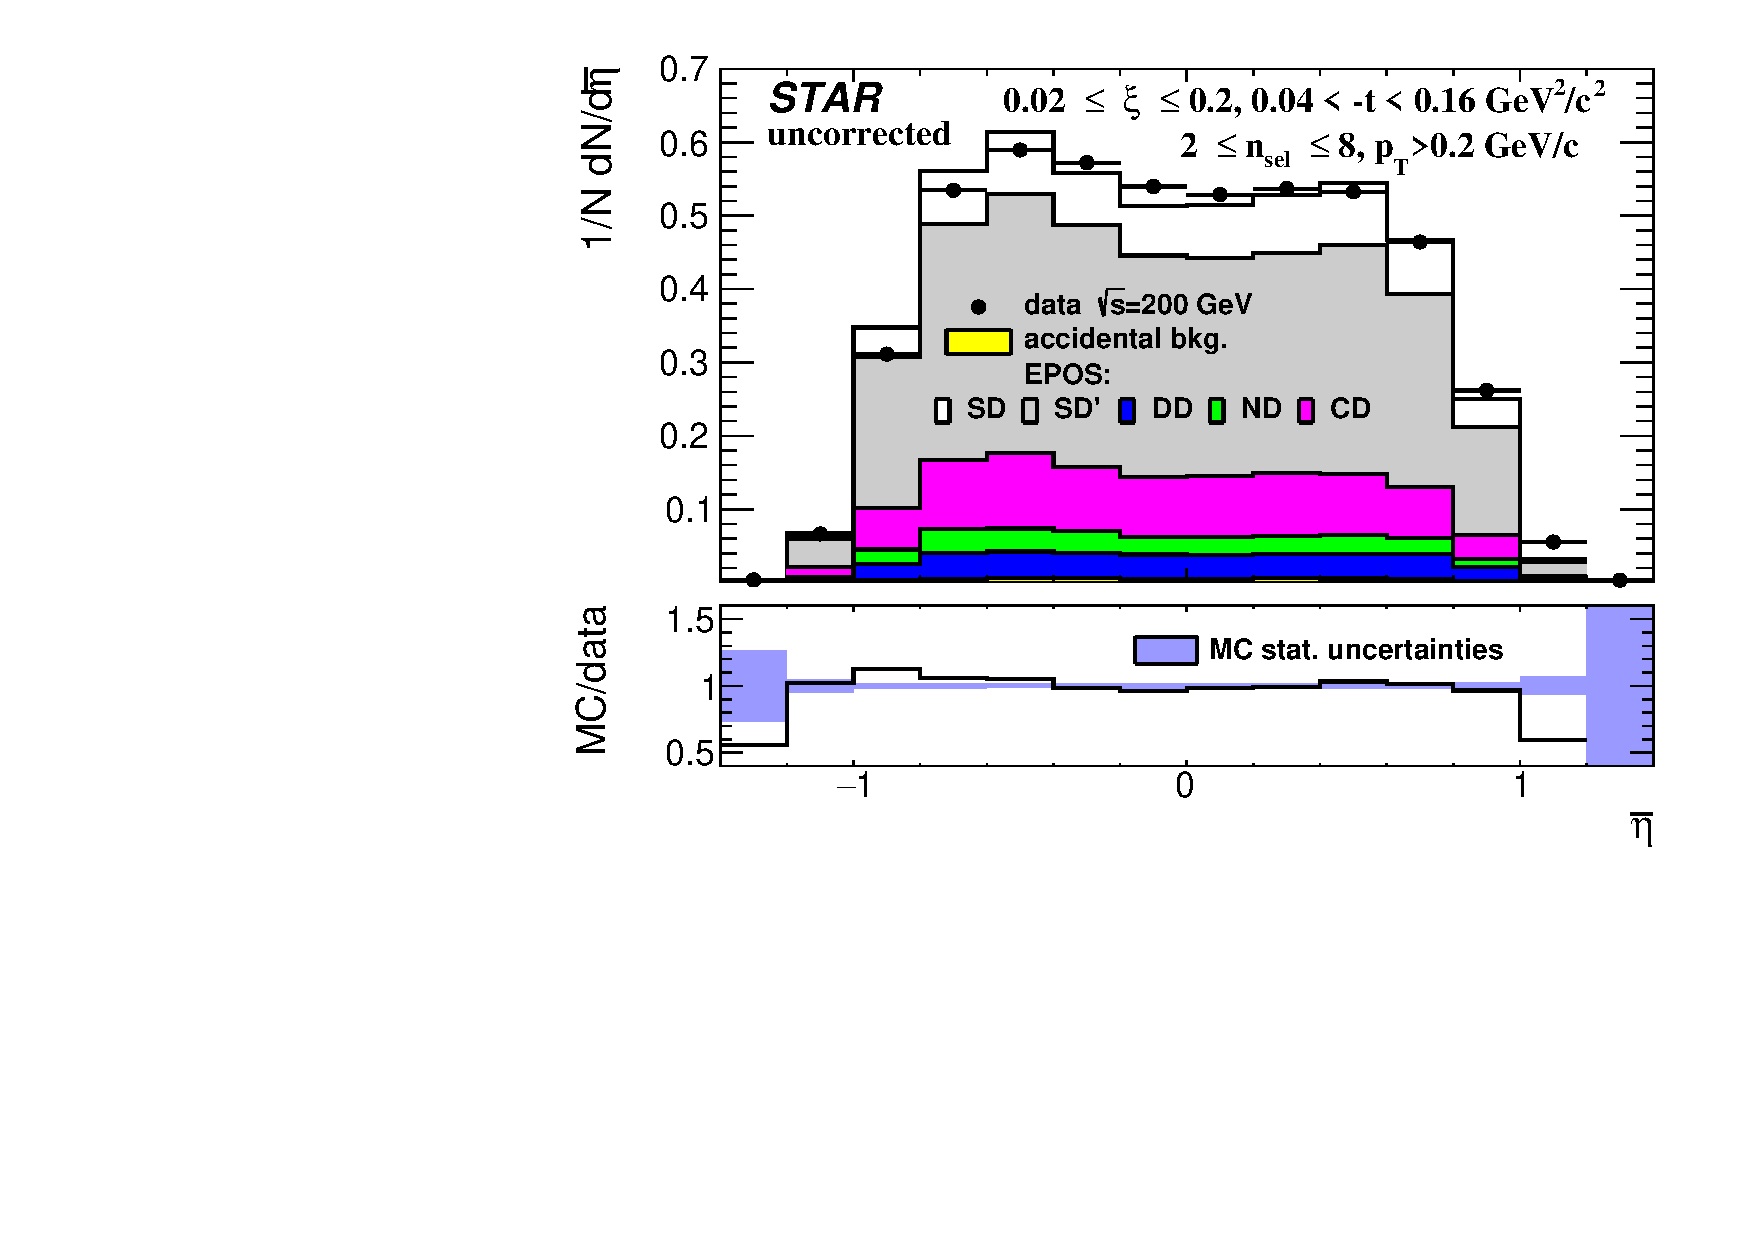
\includegraphics[width=\linewidth, page=1]{chapters/chrgSTAR/img/nonSD/chrg/SDT_epos_xi0_RP_starsim_eta.pdf}
	\end{subfigure}
	\begin{minipage}{.45\textwidth}
		\caption[Uncorrected distributions of data compared to various MC models: PYTHIA8 A2 (MBR), PYTHIA8 A2 (MBR-tuned) and EPOS, as a function of $\bar{\eta}$.]{Uncorrected distributions of data compared to various MC models: (top left) PYTHIA8 A2 (MBR), (top right) PYTHIA8 A2 (MBR-tuned) and (bottom) EPOS, as a function of $\bar{\eta}$. Both data and MC are scaled by the respective numbers of events in the samples.}
		\label{fig:nonSDera}
	\end{minipage}
	
\end{figure}
\FloatBarrier
\captionsetup{format=default,indention=0pt,justification=justified}